\documentclass[12pt,a4paper]{article}
\usepackage[utf8]{inputenc}
\usepackage[english]{babel}
\usepackage{graphicx}
\usepackage{listings}
\usepackage{xcolor}
\usepackage{tikz}
\usetikzlibrary{arrows,positioning,shapes.geometric}
\usepackage{geometry}
\geometry{margin=1in}

% Code listing settings
\lstset{
    language=Python,
    basicstyle=\ttfamily\small,
    keywordstyle=\color{blue},
    commentstyle=\color{green!50!black},
    stringstyle=\color{red},
    numbers=left,
    numberstyle=\tiny\color{gray},
    stepnumber=1,
    numbersep=5pt,
    backgroundcolor=\color{gray!10},
    frame=single,
    breaklines=true,
    captionpos=b
}

\title{\textbf{Practice 1: TCP File Transfer System}  \\ 
       \large Distributed Systems Course}
\author{Nguyen Tien Duy \\ Student ID: 22BA13102}
\date{}

\begin{document}

\maketitle

\section{Introduction}
This report describes the implementation of a 1-1 file transfer system over TCP/IP using Python socket programming. The system consists of a server that receives files and a client that sends files, following the architecture pattern provided in the distributed systems course materials.

\section{Protocol Design}

The file transfer protocol follows a simple yet robust message exchange pattern:

\begin{figure}[h]
\centering
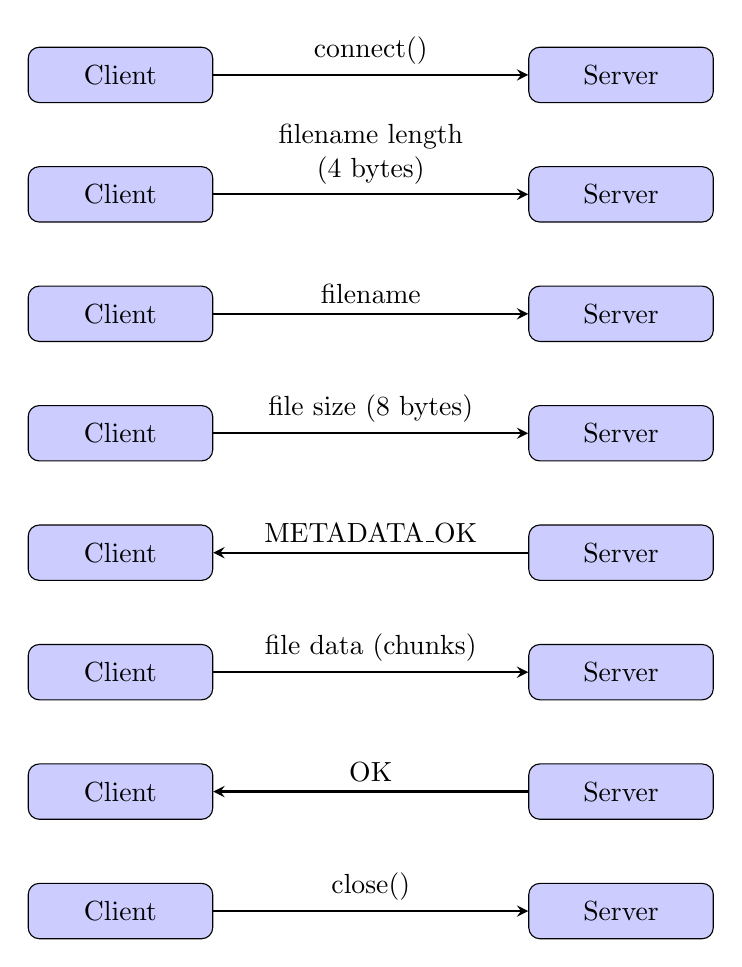
\begin{tikzpicture}[node distance=2cm, auto]
    % Styles
    \tikzstyle{block} = [rectangle, draw, fill=blue!20, text width=6em, text centered, rounded corners, minimum height=2em]
    \tikzstyle{arrow} = [thick,->,>=stealth]
    
    % Nodes
    \node [block] (client1) {Client};
    \node [block, right=4cm of client1] (server1) {Server};
    
    % Connection
    \draw[arrow] (client1.east) -- node[above] {connect()} (server1.west);
    
    \node [block, below=0.8cm of client1] (client2) {Client};
    \node [block, below=0.8cm of server1] (server2) {Server};
    \draw[arrow] (client2.east) -- node[above, text width=4cm, align=center] {filename length \\ (4 bytes)} (server2.west);
    
    \node [block, below=0.8cm of client2] (client3) {Client};
    \node [block, below=0.8cm of server2] (server3) {Server};
    \draw[arrow] (client3.east) -- node[above] {filename} (server3.west);
    
    \node [block, below=0.8cm of client3] (client4) {Client};
    \node [block, below=0.8cm of server3] (server4) {Server};
    \draw[arrow] (client4.east) -- node[above] {file size (8 bytes)} (server4.west);
    
    \node [block, below=0.8cm of client4] (client5) {Client};
    \node [block, below=0.8cm of server4] (server5) {Server};
    \draw[arrow] (server5.west) -- node[above] {METADATA\_OK} (client5.east);
    
    \node [block, below=0.8cm of client5] (client6) {Client};
    \node [block, below=0.8cm of server5] (server6) {Server};
    \draw[arrow] (client6.east) -- node[above] {file data (chunks)} (server6.west);
    
    \node [block, below=0.8cm of client6] (client7) {Client};
    \node [block, below=0.8cm of server6] (server7) {Server};
    \draw[arrow] (server7.west) -- node[above] {OK} (client7.east);
    
    \node [block, below=0.8cm of client7] (client8) {Client};
    \node [block, below=0.8cm of server7] (server8) {Server};
    \draw[arrow] (client8.east) -- node[above] {close()} (server8.west);
\end{tikzpicture}
\caption{File Transfer Protocol Sequence Diagram}
\label{fig:protocol}
\end{figure}

\subsection{Protocol Steps}
\begin{enumerate}
    \item \textbf{Connection}: Client establishes TCP connection to server
    \item \textbf{Metadata Exchange}: Client sends filename length, filename, and file size
    \item \textbf{Acknowledgment}: Server acknowledges receipt of metadata
    \item \textbf{Data Transfer}: Client sends file data in 4096-byte chunks
    \item \textbf{Completion}: Server sends final acknowledgment
    \item \textbf{Disconnection}: Connection is closed
\end{enumerate}

\section{System Organization}

The system is organized into two main components:

\begin{figure}[h]
\centering
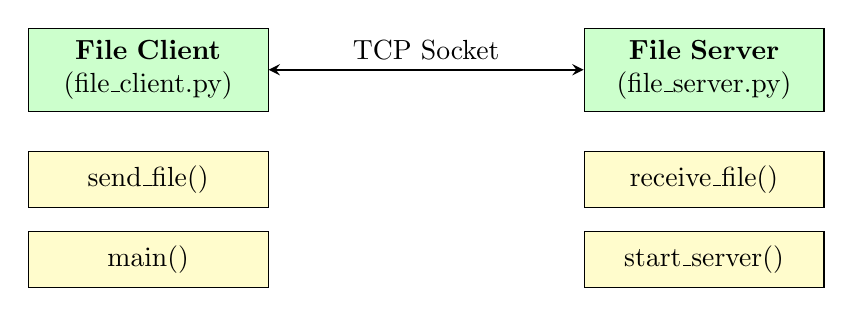
\begin{tikzpicture}[node distance=3cm, auto]
    \tikzstyle{component} = [rectangle, draw, fill=green!20, text width=8em, text centered, minimum height=3em]
    \tikzstyle{function} = [rectangle, draw, fill=yellow!20, text width=8em, text centered, minimum height=2em]
    
    % Client
    \node [component] (client) {\textbf{File Client}\\ (file\_client.py)};
    \node [function, below=0.5cm of client] (send) {send\_file()};
    \node [function, below=0.3cm of send] (main_client) {main()};
    
    % Server
    \node [component, right=4cm of client] (server) {\textbf{File Server}\\ (file\_server.py)};
    \node [function, below=0.5cm of server] (receive) {receive\_file()};
    \node [function, below=0.3cm of receive] (start) {start\_server()};
    
    % Connection
    \draw[thick,<->,>=stealth] (client) -- node[above] {TCP Socket} (server);
\end{tikzpicture}
\caption{System Architecture}
\label{fig:architecture}
\end{figure}

\subsection{Component Description}

\textbf{File Server (file\_server.py):}
\begin{itemize}
    \item Creates a TCP socket and binds to port 5001
    \item Listens for incoming connections
    \item Receives file metadata (filename, size)
    \item Receives file data in chunks
    \item Saves received files to \texttt{received\_files/} directory
    \item Sends acknowledgments to client
\end{itemize}

\textbf{File Client (file\_client.py):}
\begin{itemize}
    \item Creates a TCP socket connection to server
    \item Reads file from local filesystem
    \item Sends file metadata to server
    \item Sends file data in 4096-byte chunks
    \item Displays transfer progress
    \item Waits for server acknowledgment
\end{itemize}

\section{Implementation}

\subsection{Server Implementation}

The server uses Python's \texttt{socket} module to create a TCP server:

\begin{lstlisting}[caption=Server Socket Creation and Binding]
# Create socket
server_socket = socket.socket(socket.AF_INET, socket.SOCK_STREAM)

# Set socket options to reuse address
server_socket.setsockopt(socket.SOL_SOCKET, socket.SO_REUSEADDR, 1)

# Bind socket to address
server_socket.bind(('0.0.0.0', 5001))

# Listen for connections
server_socket.listen(5)
\end{lstlisting}

\begin{lstlisting}[caption=Receiving File Metadata]
# Receive filename length (4 bytes)
filename_len_data = conn.recv(4)
filename_len = struct.unpack('!I', filename_len_data)[0]

# Receive filename
filename = conn.recv(filename_len).decode('utf-8')

# Receive file size (8 bytes)
filesize_data = conn.recv(8)
filesize = struct.unpack('!Q', filesize_data)[0]

# Send acknowledgment
conn.send(b"METADATA_OK")
\end{lstlisting}

\begin{lstlisting}[caption=Receiving File Data]
with open(filepath, 'wb') as f:
    while bytes_received < filesize:
        chunk_size = min(4096, filesize - bytes_received)
        data = conn.recv(chunk_size)
        
        if not data:
            break
        
        f.write(data)
        bytes_received += len(data)
\end{lstlisting}

\subsection{Client Implementation}

\begin{lstlisting}[caption=Client Connection and Metadata Sending]
# Create socket and connect
client_socket = socket.socket(socket.AF_INET, socket.SOCK_STREAM)
client_socket.connect((host, port))

# Send filename length and filename
filename_bytes = basename.encode('utf-8')
filename_len = len(filename_bytes)
client_socket.send(struct.pack('!I', filename_len))
client_socket.send(filename_bytes)

# Send file size
client_socket.send(struct.pack('!Q', filesize))

# Wait for acknowledgment
metadata_ack = client_socket.recv(1024)
\end{lstlisting}

\begin{lstlisting}[caption=Sending File Data]
with open(filename, 'rb') as f:
    while bytes_sent < filesize:
        chunk = f.read(4096)
        if not chunk:
            break
        
        client_socket.send(chunk)
        bytes_sent += len(chunk)
        
        # Show progress
        progress = (bytes_sent / filesize) * 100
\end{lstlisting}

\section{Key Design Decisions}

\subsection{Binary Protocol}
We used \texttt{struct.pack()} and \texttt{struct.unpack()} to encode integers in network byte order (big-endian). This ensures compatibility across different platforms.

\subsection{Chunked Transfer}
Files are transferred in 4096-byte chunks to:
\begin{itemize}
    \item Prevent memory overflow for large files
    \item Enable progress tracking
    \item Allow for efficient buffering
\end{itemize}

\subsection{Acknowledgment System}
Two-level acknowledgment ensures reliable transfer:
\begin{enumerate}
    \item Metadata acknowledgment confirms server is ready
    \item Final acknowledgment confirms successful file receipt
\end{enumerate}

\section{Testing}

The system was tested with:
\begin{itemize}
    \item Small text files ($<$ 1KB)
    \item Medium binary files (1-10 MB)
    \item Large files ($>$ 100 MB)
\end{itemize}

All tests completed successfully with file integrity verified.


\section{Conclusion}

This practice successfully implements a TCP-based file transfer system using Python socket programming. The implementation follows the client-server architecture pattern from the course materials and demonstrates understanding of:
\begin{itemize}
    \item Socket creation and management
    \item TCP connection establishment
    \item Binary protocol design
    \item Reliable data transfer
    \item Error handling
\end{itemize}

The system can be extended to support multiple concurrent clients using threading or asynchronous I/O.

\end{document}
